% ch9.tex
% This work is licensed under the Creative Commons Attribution-Noncommercial-Share Alike 3.0 New Zealand License.
% To view a copy of this license, visit http://creativecommons.org/licenses/by-nc-sa/3.0/nz
% or send a letter to Creative Commons, 171 Second Street, Suite 300, San Francisco, California, 94105, USA.


\chapter{Algo sobre gráficos}\label{ch:abitgraphic}

El problema de utilizar una tortuga para dibujar, es$\ldots$ que$\ldots$$\ldots$ las tortugas$\ldots$$\ldots$$\ldots$ son$\ldots$$\ldots$$\ldots$$\ldots$ muy$\ldots$$\ldots$$\ldots$$\ldots$$\ldots$ lentas.
\par
Una tortuga, incluso aunque vaya a su máxima velocidad, nunca va rápida.  Para las tortugas, esto no es realmente un problema---tienen todo el tiempo del mundo---pero cuando estamos hablando de gráficos de ordenador, sí que importa.  Si tienes una Nintendo DS, una Gameboy Advance, o juegas en tu ordenado, piensa por un momento en los gráficos (lo que ves en la pantalla). Hay varias formas en las que se presentan los gráficos de los juegos: Hay juegos en 2d (en dos dimensiones), en los que las imágenes son planas y los personajes se mueven únicamente hacia arriba, abajo, izquierda o derecha---es bastante común en dispositivos portátiles como la Gameboy, Nintendo DS o teléfonos móviles.  Hay también juegos pseudo-3d (casi en tres dimensiones), en las que las imágenes parecen algo más reales, pero en los que los personajes aún se mueven únicamente hacia arriba, abajo, izquierda y derecha---de nuevo son comunes en dispositivos portátiles---y finalmente existen los juegos en 3d, en los que las imágenes de la pantalla intentan imitar la realidad (como en los simuladores de carreras de coches o de aviones en vuelo).

Todos los tipos de gráficos tienen una cosa en común---se necesita dibujarlos rápidamente en la pantalla del ordenador.  ¿Has probado a hacer tu propia animación?  Esa en la que usas un taco de hojas de papel y en la esquina de la primera página dibuas algo (tal vez un muñequito hecho de rayitas), en la esquina inferior de la siguiente página dibujas la misma figura en el mismo sitio pero le mueves la pierna un poco. Luego en la siguiente pagina dibujas la figura de nuevo con la pierna un poquito más allá. Gradualmente vas página a página dibujando la figura moviéndose en la esquina inferior del taco de páginas.  Cuando has terminado, pasas las páginas rápidamente con el dedo de forma que parece que el muñequito se está moviendo.  Así son las bases de todas las animaciones que se hacen---ya sean dibujos animados en la tele o los juegos de ordenador o consola.  Dibujas algo en pantalla y luego lo vuelves a dibujar un poco cambiado de lugar de forma que si se hace rápido parece que es la misma imagen que se está moviendo. Por es la tortuga no es buena para hacer gráficos.  Par que una imagen parezca que está en movimiento es necesario dibujar cada `frame' (cuadro) de la animación muy rápido. 
\par
Los gráficos en tres dimensiones se hacen de una forma diferente de los de dos dimensiones, pero la base de la idea es la misma.  Para cuando la tortuga ha terminado de dibujar sólo una pequeña parte de la imagen ya habría que estar pasando la página e iniciando el dibujo de la siguiente página$\ldots$

\begin{center}
\includegraphics*[width=100mm]{turtle1.eps}
\end{center}

\section{Dibujo rápido}

Cada lenguaje de programación tiene una forma (o varias) diferente de dibujar en la pantalla. Algunos métodos son rápidos y otros son lentos, lo que significa que los programadores que desarrollan juegos tienen que ser muy cuidadosos con el lenguaje en el que eligen trabajar.
\par
Python dispone de diferentes formas de dibujar gráficos (incluida la tortuga del módulo turtle que ya hemos utilizado), pero los mejores métodos (desde el punto de vista de los gráficos) están en módulos y librerías de código que no están incluidas con el propio lenguaje.  Posiblemente tendrás que programar durante varios años antes de que seas capaz de saber cómo instalar y utilizar una de estas complejas librerías.

Afortunadamente, existe un módulo, que viene con Python, que podemos utilizar para hacer gráficos (a una velocidad ligeramente superior a la tortuga). Tal vez lo suficientemente rápido como para poderlo llamar la Tortuga de dibujo veloz. 


\begin{center}
\includegraphics*[width=100mm]{turtle2.eps}
\end{center}

Este módulo se llama \code{Tkinter}\index{módulos!Tkinter} (es un nombre extraño que significa `Tk interface') y que se puede utilizar para crear aplicaciones completas (podrías incluso crar un programa de proceso de textos simple si quisieras---como un Microsoft Word sencillito). Podríamos crear una aplicación simple que muestre un botón con el siguiente código:

\begin{listing}
\begin{verbatim}
1. >>> from Tkinter import *
2. >>> ventana = Tk()
3. >>> btn = Button(ventana, text="Púlsame")
4. >>> btn.pack()
\end{verbatim}
\end{listing}

En la línea 2 importamos el contenido del módulo \code{Tk} para que podamos usarlos\footnote{La diferencia entre `import Tkinter' y `from Tkinter import *' es que con la primera sentencia se importa el módulo pero es necesario utilizar el nombre el módulo para usar las funciones y objetos que están dentro de él (Tkinter.Tk() o Tkinter.Button($\ldots$), y con la segunda sentencia se importa el módulo pero no es necesario usar el nombre del mismo para usarlas (Tk() o Button($\ldots$)}. En la segunda línea usamos una de las funciones más útiles del módulo, \code{Tk}, que crea una ventana de las que se dibujan en la pantalla a la que podemos añadir cosas.  Después de teclear la línea 2 verás que la ventana aparece instantáneamente en la pantalla. En la línea 3 creamos un objeto botón y lo asignamos a la variable \code{btn}.  El botón se crea mediante una función a la que se le pasa la ventana (el objeto creado anteriormente con Tk()) y una cadena que lleva el texto `Púlsame'.

\par
\fbox{\colorbox{PaleBlue}{\parbox{.75\linewidth} {
\section*{Parámetros con nombre}

Esta es la primera vez que hemos usado `parámetros con nombre'\index{parámetros con nombre}. Funcionan como cualquier otro parámetro con la única diferencia de que pueden aparecer en cualquier orden, es por eso por lo que hace falta proporcionarles un nombre.

Por ejemplo, supongamos que tenemos una función rectángulo que recibe dos parámetros denominados alto y ancho.  Normalmente podríamos llamar a la función utilizando algo como rectangulo(200, 100), que significa que queremos dibujar un rectángulo de 200 pixels de ancho y 100 pixels de alto. 

Si quisieramos que los parámetros pudieran escribirse en cualquier orden es necesario decir cual es cual, para ello podríamos llamar a la función de la siguiente manera: rectangulo(alto=100, ancho=200). 

La idea de los parámetros con nombre es más compleja que lo que hemos mostrado aquí, y puede utilizarse de varias formas para hacer que las funciones se puedan utilizar de formas más flexibles---pero esta es una materia para un libro más avanzado que este libro introductorio de programación.
\par
}}}
\par

La cuarta línea le indica al botón que se debe dibujar a sí mismo. En este momento, la ventana que creamos en la línea 2 se ajustará al tamaño del botón que contiene el texto `Púlsame'. Verás algo parecido a esto: 

\begin{center}
\includegraphics*[width=30mm]{figure31.eps}
\end{center}

Con lo que llevamos hecho el botón no hace nada especial, pero por lo menos lo puedes pulsar.

Vamos a hacer que haga algo modificando el ejemplo anterior un poco (asegúrate de que cierras la ventanas que creamos anteriormente). Primero creamos una función que imprima algún texto:

\begin{listing}
\begin{verbatim}
>>> def saludar():
...     print('hola')
\end{verbatim}
\end{listing}

\noindent
Ahora modificamos el ejemplo para que utilice la función que hemos creado:

\begin{listing}
\begin{verbatim}
>>> from Tkinter import *
>>> ventana = Tk()
>>> btn = Button(ventana, text="Púlsame", command=saludar)
>>> btn.pack()
\end{verbatim}
\end{listing}

El parámetro con nombre `command' sirve para indicarle al botón que tiene que ejecutar la función que se le indica cuando se pulse el botón. En nuestro caso, al pulsar el botón se escribirá el texto `hola' en la consola---cada vez que se pulse el botón. 

\section{Dibujos simples}

Los botones no son muy útiles cuando lo que quieres es dibujar en la pantalla---por eso tenemos que crear y añadir un tipo diferente de componente: el objeto \code{Canvas}\index{módulos!Tkinter!Canvas}(lienzo). A diferencia de un botón (que toma los parámetros `text' y `command') cuando creamos un lienzo (canvas), necesitamos pasarle el ancho y la altura (en píxeles) del lienzo.  Aparte de esto el resto del código es muy similar al código para mostrar un botón en pantalla:

\begin{listing}
\begin{verbatim}
>>> from Tkinter import *
>>> ventana = Tk()
>>> lienzo = Canvas(ventana, width=500, height=500)
>>> lienzo.pack()
\end{verbatim}
\end{listing}

Como en el caso del botón, al escribir la línea 2 se muestra una ventana en pantalla. La empaquetar (`pack') el lienzo en la línea cuatro se incrementará su tamaño para que quepa el lienzo (de 500x500) en la ventana.

Ahora podemos dibujar una línea en el lienzo utilizando las coordenadas de los píxeles.  Las coordenadas indican la posición de los píxeles en un lienzo.  En un lienzo del módulo Tk, las coordenadas indican la distancia del los píxeles en relación con la esquina superior izquierda del mismo. En otras palabras, el pixel 0,0 está situado en la esquina superior izquierda del lienzo.  

Del valor que sirve para medir la distancia de izquierda a derecha se dice que mide la distancia sobre el eje x (izquierda a derecha).  Del valor que sirve para medir la distancia de arriba a abajo se dice que mide la distancia sobre el eje y (arriba a abajo).

\begin{figure}
\begin{center}
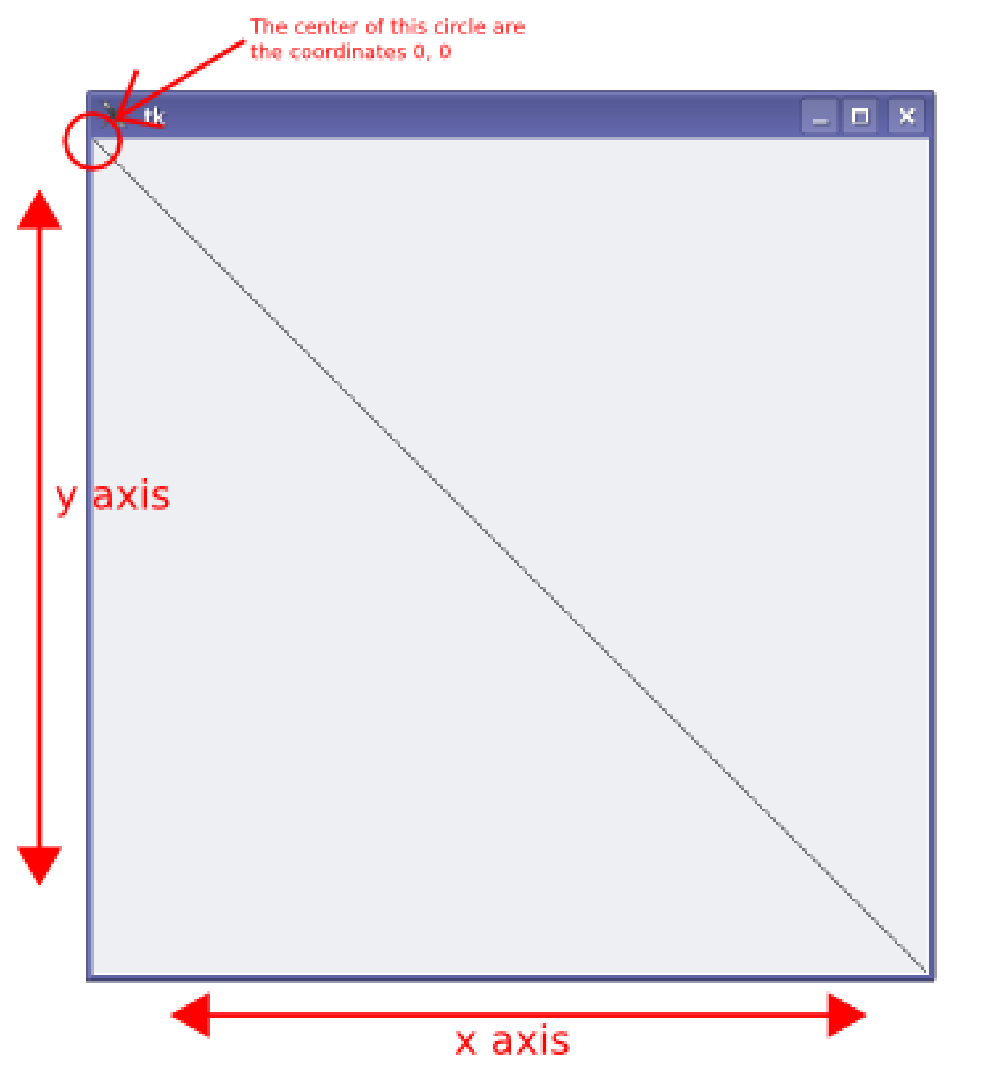
\includegraphics[width=80mm]{figure32.eps}
\end{center}
\caption{Lienzo y ejes x e y.}\label{fig32}
\end{figure}

Puesto que el lienzo que hemos creado mide 500 píxeles de ancho y 500 píxeles de alto, las coordenadas de la esquina inferior derecha de la pantalla es 500,500. Por eso, la línea que se muestra en la figura~\ref{fig32} hay que dibujarla utilizando las coordenadas 0,0 como lugar de inicio y las 500,500 como final\index{módulos!Tkinter!create\_line}:

\begin{listing}
\begin{verbatim}
>>> from Tkinter import *
>>> ventana = Tk()
>>> lienzo = Canvas(ventana, width=500, height=500)
>>> lienzo.pack()
>>> lienzo.create_line(0, 0, 500, 500)
\end{verbatim}
\end{listing}

\noindent
Para hacer lo mismo con el módulo turtle hubieramos necesitado el código siguiente:

\begin{listing}
\begin{verbatim}
>>> import turtle
>>> turtle.setup(width=500, height=500)
>>> t = turtle.Pen()
>>> t.up()
>>> t.goto(-250,250)
>>> t.down()
>>> t.goto(500,-500)
\end{verbatim}
\end{listing}

Como se puede ver el código del módulo Tkinter es un mejora al ser más corto y menos complejo. En el objeto canvas (lienzo) existen muchos métodos (funciones) disponibles, algunos de ellos no nos son muy útiles en este momento, pero vamos a echar un vistazo a algunos ejemplos con funciones que sí que son interesantes.

\section{Dibujando cajas}

En la tortuga teníamos que dibujar una caja avanzando y girando varias veces. Con Tkinter dibujar un cuadrado o rectángulo es bastante más fácil---únicamente necesitas indicar las coordenadas de las esquinas.

\begin{listingignore}
\begin{verbatim}
>>> from Tkinter import *
>>> ventana = Tk()
>>> lienzo = Canvas(ventana, width=400,height=400)
>>> lienzo.pack()
>>> lienzo.create_rectangle(10, 10, 50, 50)
1
\end{verbatim}
\end{listingignore}

En el ejemplo anterior, creamos un lienzo de 400 píxeles de ancho y 400 píxeles de alto. Después dibujamos un cuadrado en la esquina superior izquierda (la esquina superior izquierda del cuadrado esta a 10 píxeles de la esquina superior izquierda, y la esquina inferior derecha está en la posición 50,50).  Si te estás preguntando qué es el número que aparece en la consola después de teclear el código \code{create\_rectangle}\index{módulos!Tkinter!create\_rectange} y antes cuando utilizamos \code{create\_line}, te explico que es un número de identificación para la figura que has dibujado (sea una línea, un cuadrado o un círculo). Volveremos este número más adelante.

De acuerdo con lo explicado, los parámetros que se utilizar para \code{create\_rectangle} son: la esquina superior izquierda (primer y segundo parámetros: posición sobre el eje X y posición sobre el eje Y) del cuadrado, y la esquina inferior derecha del cuadrado (tercer y cuarto parámetro: posición sobre eje X y posición sobre eje Y). En adelante, para no tener que explicarlo mucho, nos referiremos a estas coordenadas como x1, y1 y x2, y2. 

Podemos dibujar un rectángulo simplemente haciendo x2 más grande:

\begin{listing}
\begin{verbatim}
>>> lienzo.create_rectangle(100, 100, 300, 50)
\end{verbatim}
\end{listing}

\noindent
O haciendo y2 un poco más grande:

\begin{listing}
\begin{verbatim}
>>> lienzo.create_rectangle(100, 200, 150, 350)
\end{verbatim}
\end{listing}

Vamos a explicar este último ejemplo: le decimos al lienzo que cree un rectángulo empezando con la esquina superior izquierda en la posición que comienza en el píxel 100,200 contando desde el borde de la izquierda del lienzo para el primer número y desde el borde de arriba del lienzo para el segundo número. Y que termine el rectángulo en el píxel 150,350 (también contando desde los bordes izquierdo y superior).  Con ello, debería verse algo como lo que aparece en la figura~\ref{fig33}.

\begin{figure}
\begin{center}
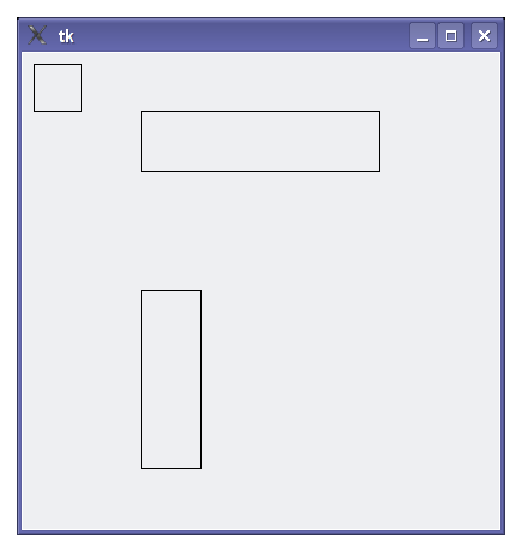
\includegraphics[width=80mm]{figure33.eps}
\end{center}
\caption{Cajas usando Tkinter.}\label{fig33}
\end{figure}

Vamos a intentar crear rectángulos de diferentes tamaños.  Para no tener que dar los tamaños nosotros mismos, vamos a usar un módulo que se llama \code{random}\index{módulos!random}. Para usarlo, en primer lugar vamos a importar el módulo random \footnote{En inglés `random' significa `aleatorio'}:

\begin{listing}
\begin{verbatim}
>>> import random
\end{verbatim}
\end{listing}

Ahora podemos crear una función que utilice números aleatorios para identificar las posiciones en las que crear los rectángulos.  Para ello tenemos que utilizar la función \code{randrange}\index{módulos!random!randrange}:

\begin{listing}
\begin{verbatim}
>>> def rectangulo_aleatorio(lienzo, ancho, alto):
...     x1 = random.randrange(ancho)
...     y1 = random.randrange(alto)
...     x2 = x1 + random.randrange(ancho-x1)
...     y2 = y1 + random.randrange(alto-y1)
...     lienzo.create_rectangle(x1, y1, x2, y2)
\end{verbatim}
\end{listing}

La función recibe el alto y el ancho del lienzo para que los rectángulos que se dibujen en pantalla sean como máximo de ese tamaño. Además recibe el lienzo en el que queremos que se dibuje el rectángulo.  La función \code{randrange} recibe un número como argumento (parámetro) (mira el Apéndice~\ref{app:afewpythonmodules} para ver más usos de \code{randrange})---así \code{randrange(10)} retorna un número entre 0 y 9, \code{randrange(100)} retorna un número entre 0 y 99, y así sucesivamente. 

Las líneas que asignan las variables x1 e y1 utilizan \code{randrange} para establecer la posición superior izquierda del rectángulo.

Las líneas que asignan las variables x2 e y2 también utilizan \code{randrange} pero primero restan los valores calculados como esquina superior izquierda antes de calcular el número aleatorio para que el rectángulo no pueda ser más grande que el ancho de la pantalla. El número así calculado será el tamaño en píxeles del rectángulo, si le sumamos la posición de inicio tendremos la posición de fin del rectángulo.

Finalmente llamamos a la función \code{create\_rectangle} con las variables creadas.  Puedes probar el código utilizando la función creada pasándole el ancho y alto del lienzo creado:

\begin{listing}
\begin{verbatim}
>>> rectangulo_aleatorio(400, 400)
\end{verbatim}
\end{listing}

\noindent
Para que aparezcan muchos en pantalla, crearíamos un bucle:

\begin{listing}
\begin{verbatim}
>>> for x in range(0, 100):
...     rectangulo_aleatorio(400, 400)
\end{verbatim}
\end{listing}

\noindent
Lo que genera un lienzo un poco embarullado (figura~\ref{fig34}.

\begin{figure}
\begin{center}
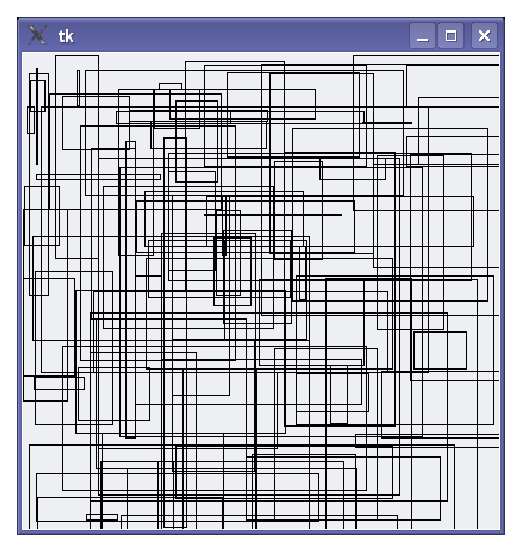
\includegraphics[width=80mm]{figure34.eps}
\end{center}
\caption{Un barullo de rectángulos.}\label{fig34}
\end{figure}

¿Recuerdas cuando en el anterior capítulo le decíamos a la tortuga que dibujase con diferentes colores utilizando porcentajes de 3 colores: rojo, verde y azul? Con el módulo Tkinter puedes hacer algo similar, pero desafortunadamente, es algo más complejo que con el módulo turtle.  En primer lugar vamos a modificar la función que genera rectángulos aleatorios para pasarle como parámetro el color con el que queremos rellenar el rectángulo que se genere:

\begin{listing}
\begin{verbatim}
>>> def rectangulo_aleatorio(lienzo, ancho, alto, color_relleno):
...     x1 = random.randrange(ancho)
...     y1 = random.randrange(alto)
...     x2 = x1 + random.randrange(ancho-x1)
...     y2 = y1 + random.randrange(alto-y1)
...     lienzo.create_rectangle(x1, y1, x2, y2, fill=color_relleno)
\end{verbatim}
\end{listing}

La función \code{create\_rectangle} del lienzo puede recibir el parámetro `fill' que sirve para especificarle el color de relleno.  Ahora podemos pasar el color de relleno a la función de la siguiente forma. Prueba lo siguiente:

\begin{listing}
\begin{verbatim}
>>> rectangulo_aleatorio(400, 400, 'green')
>>> rectangulo_aleatorio(400, 400, 'red')
>>> rectangulo_aleatorio(400, 400, 'blue')
>>> rectangulo_aleatorio(400, 400, 'orange')
>>> rectangulo_aleatorio(400, 400, 'yellow')
>>> rectangulo_aleatorio(400, 400, 'pink')
>>> rectangulo_aleatorio(400, 400, 'purple')
>>> rectangulo_aleatorio(400, 400, 'violet')
>>> rectangulo_aleatorio(400, 400, 'magenta')
>>> rectangulo_aleatorio(400, 400, 'cyan')
\end{verbatim}
\end{listing}

Algunos, puede que todos, los nombres de colores funcionarán. Pero algunos de ellos podrían dar como resultado un mensaje de error (depende de que estés utilizando Windows, Mac OS X o Linux). Por ahora es muy sencillo. Pero ¿cómo hacemos para dibujar con el color dorado?  En el módulo de la tortuga utilizamos las mezclas de luz de colores.  En \code{Tkinter} podemos crear el dorado utilizando:

\begin{listing}
\begin{verbatim}
>>> rectangulo_aleatorio(400, 400, '#ffd800')
\end{verbatim}
\end{listing}

Lo que es una forma muy extraña de crear un color. `ffd800' es un número hexadecimal\index{colores hexadecimales}, que sirve para representar números de forma diferente a como solemos hacerlo.  Explicar cómo funcionan los números decimales nos llevaría muchas páginas, así que por el momento, puedes utilizar la siguiente función para crear un color en hexadecimal:

\begin{listing}
\begin{verbatim}
>>> def hexcolor(rojo, verde, azul):
...     r = 255*(rojo/100.0)
...     g = 255*(verde/100.0)
...     b = 255*(azul/100.0)
...     return '#%02x%02x%02x' % (r, g, b)
\end{verbatim}
\end{listing}

Si llamamos a la función hexcolor con 100\% para el rojo, 85\% para el verde y 0\% para el azul, el resultado es el número hexadecimal para el color dorado:

\begin{listing}
\begin{verbatim}
>>> print(hexcolor(100, 85, 0))
#ffd800
\end{verbatim}
\end{listing}

\noindent
Puedes crear un color púrpura brillante utilizando 98\% de rojo, 1\% de verde, y 77\% de azul:

\begin{listing}
\begin{verbatim}
>>> print(hexcolor(98, 1, 77))
#f902c4
\end{verbatim}
\end{listing}

\noindent
Puedes utilizarlo como parámetro de la función rectangulo\_aleatorio que creamos anteriormente: 

\begin{listing}
\begin{verbatim}
>>> rectangulo_aleatorio(400, 400, hexcolor(98, 1, 77))
\end{verbatim}
\end{listing}

\begin{figure}
\begin{center}
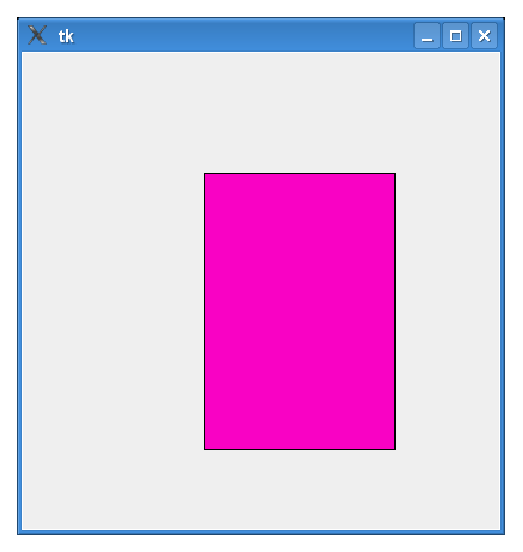
\includegraphics[width=80mm]{figure35.eps}
\end{center}
\caption{Un rectángulo púrpura.}\label{fig35}
\end{figure}

\section{Dibujando arcos}

Un arco es un trozo de un círculo, pero para dibujarlo con Tkinter lo que tienes que hacer es dibujar un rectángulo. Lo que no parece que tenga mucho sentido. Tal vez si ves la figura~\ref{fig36} te lo aclare un poco. El rectángulo indica a Tkinter el espacio que tiene para dibujar el arco.  El código para dibujar este arco sería así\index{módulos!Tkinter!create\_arc}:

\begin{listing}
\begin{verbatim}
lienzo.create_arc(10, 10, 200, 100, extent=180, style=ARC)
\end{verbatim}
\end{listing}

\begin{figure}
\begin{center}
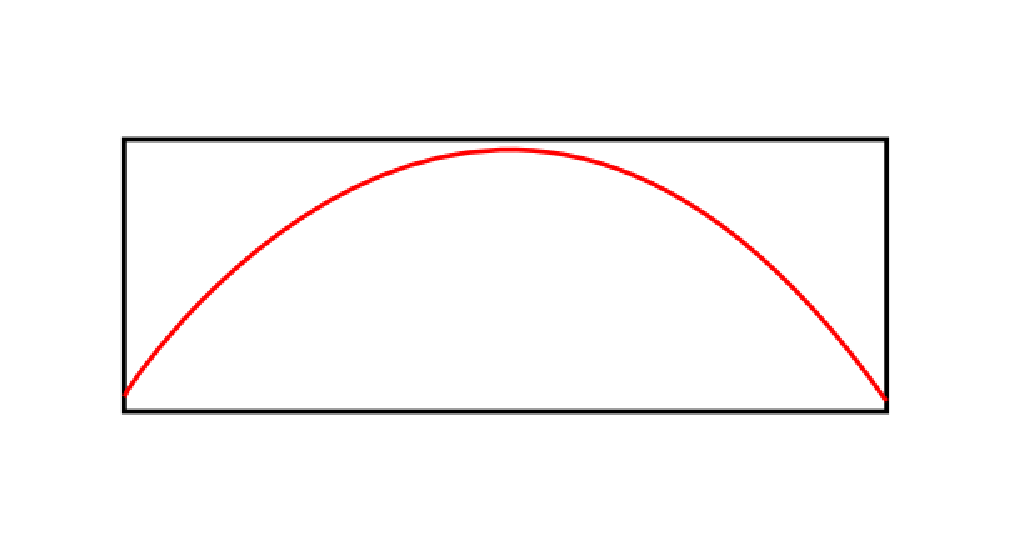
\includegraphics[width=80mm]{figure36.eps}
\end{center}
\caption{Un arco ajustado dentro de un rectángulo.}\label{fig36}
\end{figure}

Esta sentencia establece que el espacio rectangular en el que se va a dibujar el arco tiene la esquina en las coordenadas 10, 10 (10 píxeles a la derecha del borde izquierdo y 10 píxeles hacia abajo desde el borde de arriba), y la esquina inferior derecha del espacio rectangular estará en las coordenadas 200, 100 (200 píxeles a la derecha y 100 píxeles hacia abjo de los bordes izquierdo y superior).  El siguiente parámetro (un \textbf{parámetro con nombre}) `extent' se utiliza para especificar los grados de ángulo del arco.  Si no conoces nada sobre grados en un círculo (o arco), recuerda lo que hablamos sobre los círculos, 180 grados sería la mitad del círculo.  359 grados sería el círculo casi completo, 90 grados un cuarto del círculo y 0 grados sería$\ldots$ bueno, nada de nada. 

A continuación se muestra código que dibuja un puñado de arcos diferentes para que puedas ver las diferencias básicas existentes al usar diferentes grados (puedes ver los ejemplos en la figura~\ref{fig37}):

\begin{listing}
\begin{verbatim}
>>> lienzo.create_arc(10, 10, 200, 80, extent=45, style=ARC)
>>> lienzo.create_arc(10, 80, 200, 160, extent=90, style=ARC)
>>> lienzo.create_arc(10, 160, 200, 240, extent=135, style=ARC)
>>> lienzo.create_arc(10, 240, 200, 320, extent=180, style=ARC)
>>> lienzo.create_arc(10, 320, 200, 400, extent=359, style=ARC)
\end{verbatim}
\end{listing}

\begin{figure}
\begin{center}
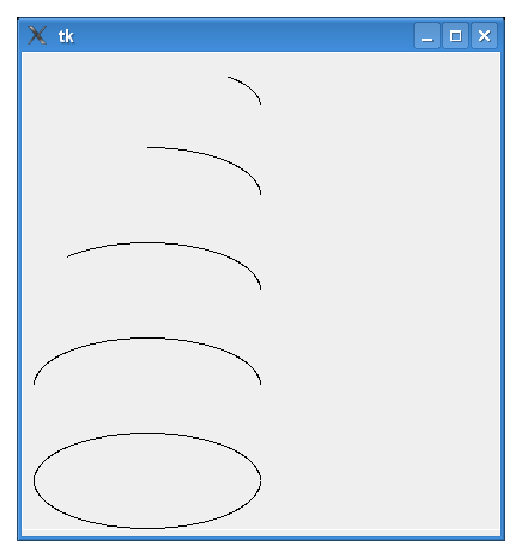
\includegraphics[width=80mm]{figure37.eps}
\end{center}
\caption{Arcos de diferentes grados.}\label{fig37}
\end{figure}

\section{Dibujando óvalos}

Aunque la última sentencia del ejemplo anterior acaba dibujando un óvalo, existe una función de Tkinter que permite dibujar un óvalo directamente. Se llama \code{create\_oval} \index{módulos!Tkinter!create\_oval}.  Del mismo modo que se dibujan los arcos, los óvalos de dibujan dentro de los límites de un rectángulo.  Por ejemplo, el código siguiente:

\begin{listing}
\begin{verbatim}
>>> ventana = Tk()
>>> lienzo = Canvas(ventana, width=400,height=400)
>>> lienzo.pack()
>>> lienzo.create_oval(1, 1, 300, 200)
\end{verbatim}
\end{listing}

Este ejemplo dibuja un óvalo dentro del rectángulo (imaginario) que va desde las posiciones 1,1 a la 300,200.  Si dibujáramos un rectánculo rojo con las mismas coordenadas lo veríamos claramente (figura~\ref{fig38}):

\begin{listing}
\begin{verbatim}
>>> lienzo.create_rectangle(1, 1, 300, 200, outline="#ff0000")
\end{verbatim}
\end{listing}

\begin{figure}
\begin{center}
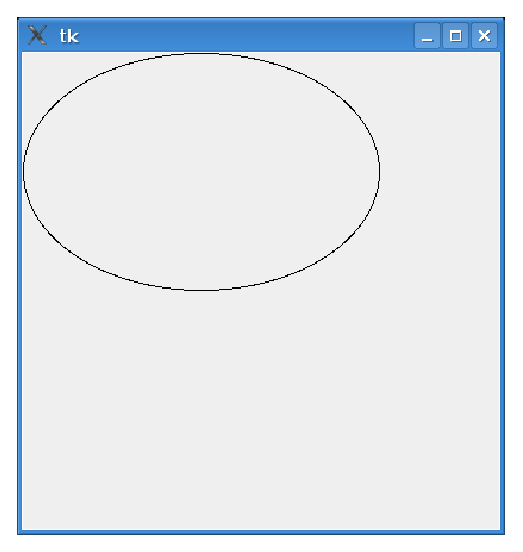
\includegraphics[width=80mm]{figure38.eps}
\end{center}
\caption{El dibujo de un óvalo.}\label{fig38}
\end{figure}

\begin{figure}
\begin{center}
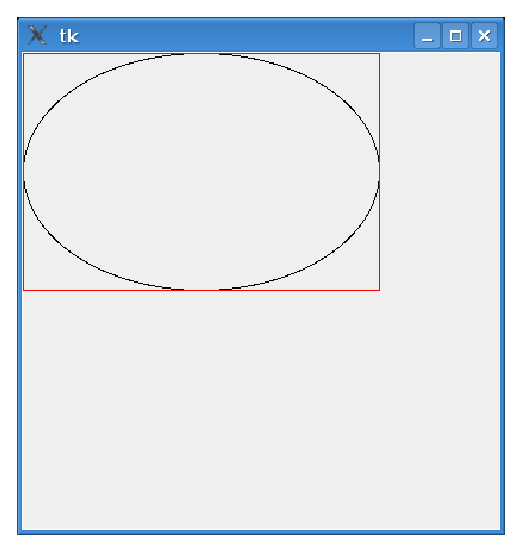
\includegraphics[width=80mm]{figure39.eps}
\end{center}
\caption{El dibujo de un óvalo dentro de un rectángulo.}\label{fig39}
\end{figure}

\noindent
Para dibujar un círculo, en lugar de un óvalo elíptico, el rectángulo `imaginario' debería ser un cuadrado (lo que genera un círculo como el de la figura~\ref{fig40}):

\begin{listing}
\begin{verbatim}
>>> ventana = Tk()
>>> lienzo = Canvas(ventana, width=400,height=400)
>>> lienzo.pack()
>>> lienzo.create_oval(1, 1, 300, 300)
\end{verbatim}
\end{listing}

\begin{figure}
\begin{center}
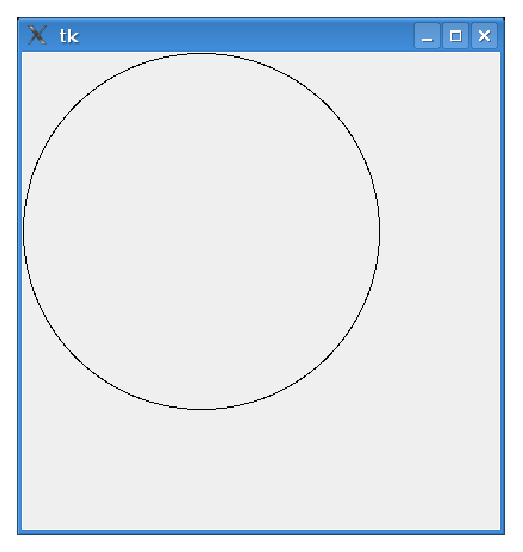
\includegraphics[width=80mm]{figure40.eps}
\end{center}
\caption{Un simple círculo.}\label{fig40}
\end{figure}

\section{Dibujando polígonos}\index{módulos!Tkinter!create\_polygon}

Un polígono es cualquier forma geométrica de 3 o más lados. Los triángulos, cuadrados, rectángulos, pentágonos y hexágonos son ejemplos de polígonos.  Además de estas formas más o menos normales, existen polígonos con formas irregulares.

Para dibujarlos con el módulo Tkinter se usa la función \code{create\_polygon}. Por ejemplo, para dibujar un triángulo tienes que proporcionar tres conjuntos de coordenadas (tres posiciones x,y), una para cada esquina del triángulo. El siguiente código crea el triángulo de la figura~\ref{fig41}):

\begin{listing}
\begin{verbatim}
>>> from Tkinter import *
>>> ventana = Tk()
>>> lienzo = Canvas(ventana, width=400,height=400)
>>> lienzo.pack()
>>> lienzo.create_polygon(10, 10, 100, 10, 100, 50, fill="", outline="black")
\end{verbatim}
\end{listing}

\begin{figure}
\begin{center}
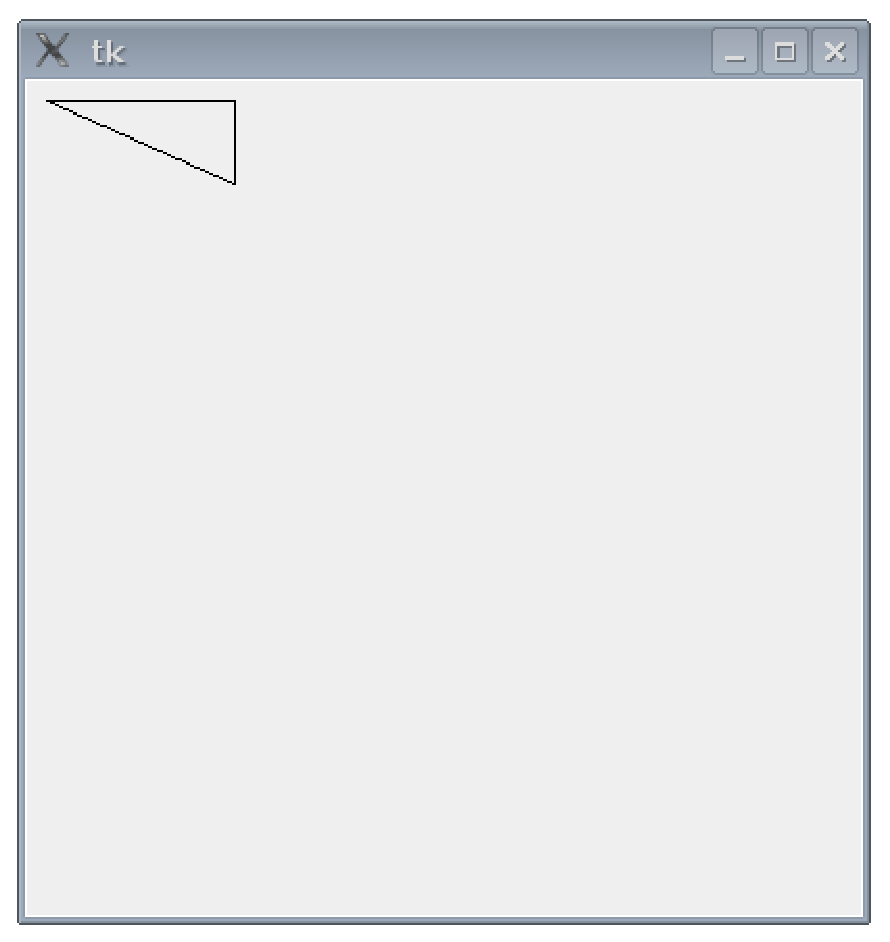
\includegraphics[width=80mm]{figure41.eps}
\end{center}
\caption{Un simple triángulo.}\label{fig41}
\end{figure}

El siguiente código genera un polígono irregular. La figura ~\ref{fig42} muestra los dos ejemplos, el triángulo y el polígono irregular.

\begin{listing}
\begin{verbatim}
>>> canvas.create_polygon(200, 10, 240, 30, 120, 100, 140, 120, fill="", outline="black")
\end{verbatim}
\end{listing}

\begin{figure}
\begin{center}
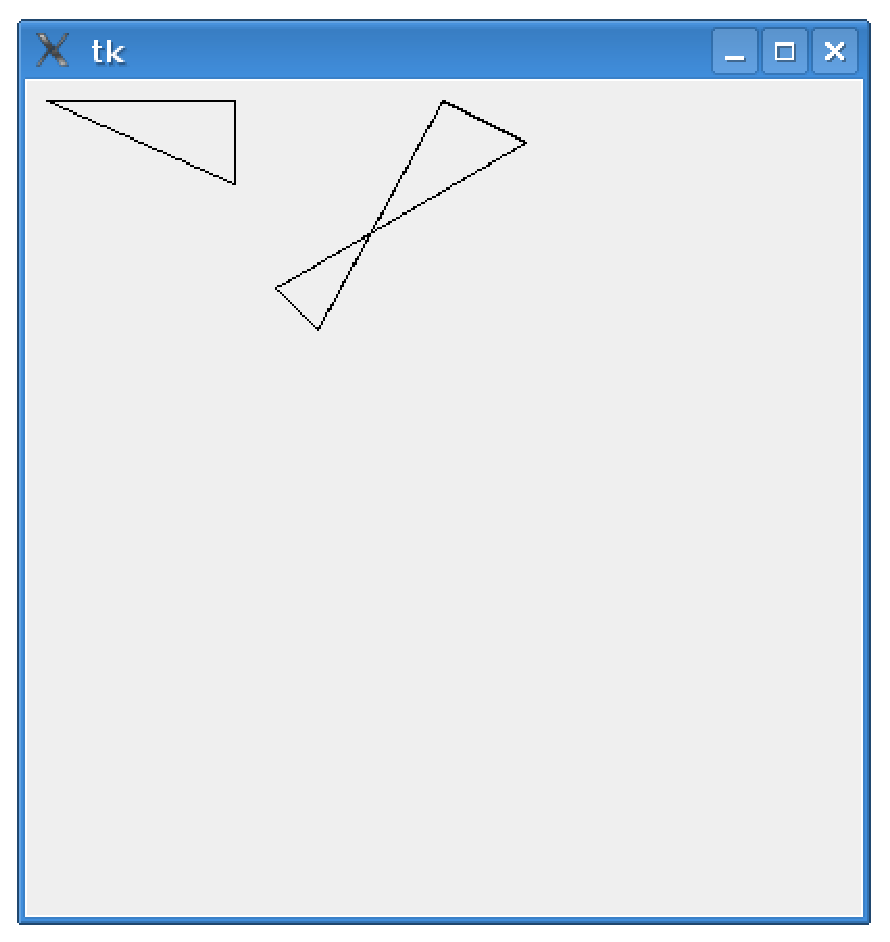
\includegraphics[width=80mm]{figure42.eps}
\end{center}
\caption{Un polígono irregular junto a un triángulo.}\label{fig42}
\end{figure}

\section{Mostrando imágenes}

También puedes mostrar una imagen en un lienzo utilizando \code{Tkinter}. En primer lugar tienes que cargar la imagen (normalmente la tendrás que tener ya en un fichero tu ordenador), luego se utiliza la función \code{create\_image}\index{módulos!Tkinter!create\_image} del objeto lienzo. Para que lo entiendas mejor el código queda como sigue:

\begin{listing}
\begin{verbatim}
1. >>> from Tkinter import *
2. >>> ventana = Tk()
3. >>> lienzo = Canvas(ventana, width=400, height=400)
4. >>> lienzo.pack()
5. >>> mi_imagen = PhotoImage(file='test.gif')
6. >>> lienzo.create_image(0, 0, image=mi_imagen, anchor=NW)
\end{verbatim}
\end{listing}

Las líneas de la 1 a la 4 crean el lienzo tal y como hemos hecho en ejemplos anteriores. En la línea 5 se carga la imagen en la variable \code{mi\_imagen}.  Es muy importante que la imagen que quieres cargar se encuentre un directorio que esté accesible para Python. Normalmente, esto supone que la imagen tiene que estar en el mismo directorio en el que arrancaste la consola. También puedes poner el path completo hasta el fichero, pero esto no lo vamos a explicar aquí.  Para saber el nombre del directorio en el que puedes poner el fichero con la imagen para que Python la pueda cargar puedes utilizar la función \code{getcwd()} del módulo \code{os}\index{módulos!os}. Como se trata de un módulo, tienes que importarlo con `import os':

\begin{listing}
\begin{verbatim}
>>> import os
>>> print(os.getcwd())
\end{verbatim}
\end{listing}

\begin{WINDOWS}
Este código imprimirá en la consola algo como `c:\\Python30'.
\end{WINDOWS}

\begin{MAC}
Este código imprimirá en consola algo como `/Users/tunombre'$\ldots$, por lo que si tu nombre es Miguel Pérez, \code{getcwd()} podría retornar algo así `/Users/miguelperez'.
\end{MAC}

\begin{LINUX}
Este código imprimirá en consola algo como `/home/tunombre'$\ldots$, por lo que si tu nombre es Miguel Pérez, \code{getcwd()} podría retorna algo como `/home/miguel' or `/home/miguelperez', dependiendo de la configuración de tu ordenador.
\end{LINUX}

Copia tu imagen en el directorio y luego cárgala utilizando la función PhotoImage (como en la línea 5) de Tkinter. Después utiliza la función \code{create\_image} para que se muestre la imagen en el lienzo (línea 6). Si has hecho todo esto correctamente, verás algo como lo de la figura~\ref{fig43}.

\begin{figure}
\begin{center}
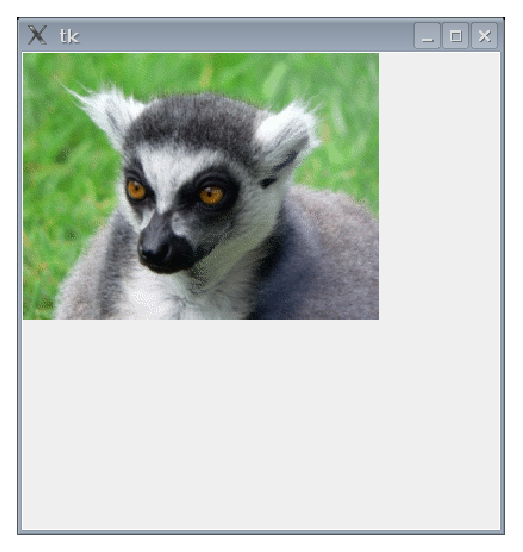
\includegraphics[width=80mm]{figure43.eps}
\end{center}
\caption{Una foto.}\label{fig43}
\end{figure}

La función PhotoImage puede cargar imágenes de archivos con las extensiones .gif, .ppm y pgm. Si quieres cargar otros tipos de imágenes (hay otros muchas formas de crear ficheros de imágenes---por ejemplo, las cámaras digitales suelen almacenar las imágenes con extensiones .jpg), necesitarás utilizar una extensión de Python que añada esta característica.  La Librería para imágenes de Python (PIL: Python Imagin Library)\footnote{La Python Imagin Library se puede descargar de \href{http://www.pythonware.com/products/pil/index.htm}{http://www.pythonware.com/products/pil/index.htm}} añade la capacidad de cargar todo tipo de imágenes, así como hacer cosas como agrandarlas o encogerlas, cambiarle los colores, invertirlas y otras muchas posibilidades. Sin embargo, instalar esta librería va más allá del ámbito de este libro.

\section{Animación básica}\index{módulos!Tkinter!animación básica}

Hasta ahora hemos visto como hacer dibujos estáticos---imágenes que no se mueven.  ¿Qué te parece hacer algo de animación? La animación no es algo en lo que \code{Tk} sea muy potente, pero podemos probar algo básico.  Por ejemplo, podemos crear un triángulo relleno y luego moverlo por la pantalla con el siguiente código:

\begin{listingignore}
\begin{verbatim}
1.  >>> import time
2.  >>> from Tkinter import *
3.  >>> ventana = Tk()
4.  >>> lienzo = Canvas(ventana, width=400, height=400)
5.  >>> lienzo.pack()
6.  >>> lienzo.create_polygon(10, 10, 10, 60, 50, 35)
7.  1
8.  >>> for x in range(0, 60):
9.  ...     lienzo.move(1, 5, 0)
10. ...     ventana.update()
11. ...     time.sleep(0.05)
\end{verbatim}
\end{listingignore}

Cuando pulses la tecla Intro después de teclear la última línea, el triángulo comenzará a moverse por la pantalla (puedes verla a mitad de camino en la figura~\ref{fig44}).

\begin{figure}
\begin{center}
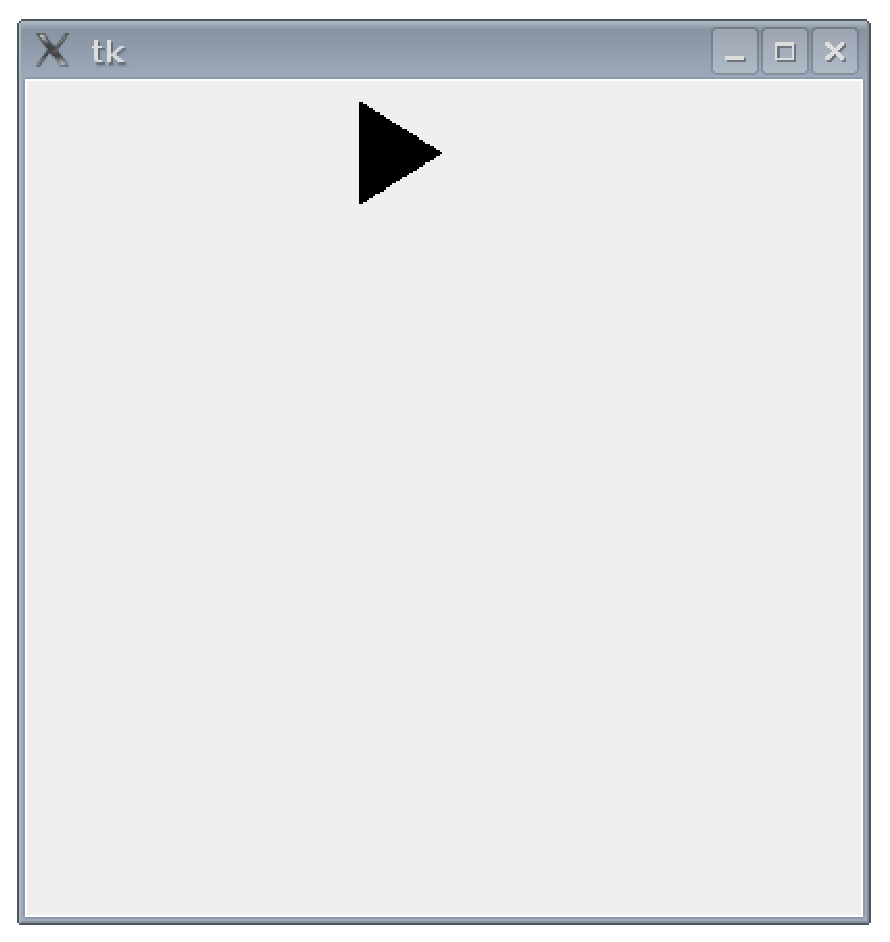
\includegraphics[width=80mm]{figure44.eps}
\end{center}
\caption{El triángulo moviéndose por la pantalla.}\label{fig44}
\end{figure}

\par
\emph{¿Cómo funciona?}
\par
Las líneas 1 a 4 las hemos visto antes---es la inicialización típica para mostrar un lienzo---en la línea 6 creamos el triángulo (utilizando la función \code{create\_polygon}). La línea 7 muestra el identificador (el número 1) que devuelve la función anterior. En la línea 8 creamos un bucle for que se repite de 0 a 59 (60 veces en total).

El bloque de líneas (9 a 11) es el código para mover el triángulo. La función \code{move} del lienzo moverá un objeto sumándole los parámetros a las coordenadas x e y actuales del objeto.  Por ejemplo, en la línea 9 lo que se está diciendo es que se mueva el objeto con el identificador 1 (el triángulo) 5 píxeles en horizontal y 0 píxeles en vertical.  Si quisiéramos que se volviera a la posición anterior tendríamos que usar números negativos \code{lienzo.move(1, -5, 0)}\index{módulos!Tkinter!move}.
 
La función \code{update} del objeto \code{ventana} obliga a actualizarla (si no usáramos dicha función, Tkinter esperaría hasta que el bucle hubiera terminado antes de mover el triángulo, lo que significaría que no lo verías moverse). Finalmente la línea 11 le dice a Python que duerma durante un fracción de segundo (un veinteavo de segundo: 1/20 = 0.05) antes de seguir. Podemos cambiar el tiempo (el parámetro de la función sleep) para que el triángulo se mueva más rápido o más lento.

También podemos modificar el código para que el triángulo se mueva en diagonal, simplemente modificando la función move: \code{move(1,5,5)}.  Primero, cierra el lienzo (pulsando el botón X de la ventana), y luego prueba este código:

\begin{listingignore}
\begin{verbatim}
>>> import time
>>> ventana = Tk()
>>> lienzo = Canvas(ventana, width=400, height=400)
>>> lienzo.pack()
>>> lienzo.create_polygon(10, 10, 10, 60, 50, 35)
1
>>> for x in range(0, 60):
...     lienzo.move(1, 5, 5)
...     tk.update()
...     time.sleep(0.05)
...
\end{verbatim}
\end{listingignore}

En la figura~\ref{fig45} se muestra el triángulo a mitad de camino de la pantalla. Paa mover el triángulo hacia arriba de la pantlla a su lugar inicial hay que utilizar el movimiento en negativo, -5, -5:

\begin{listing}
\begin{verbatim}
>>> import time
>>> for x in range(0, 60):
...     lienzo.move(1, -5, -5)
...     tk.update()
...     time.sleep(0.05)
\end{verbatim}
\end{listing}

\begin{figure}
\begin{center}
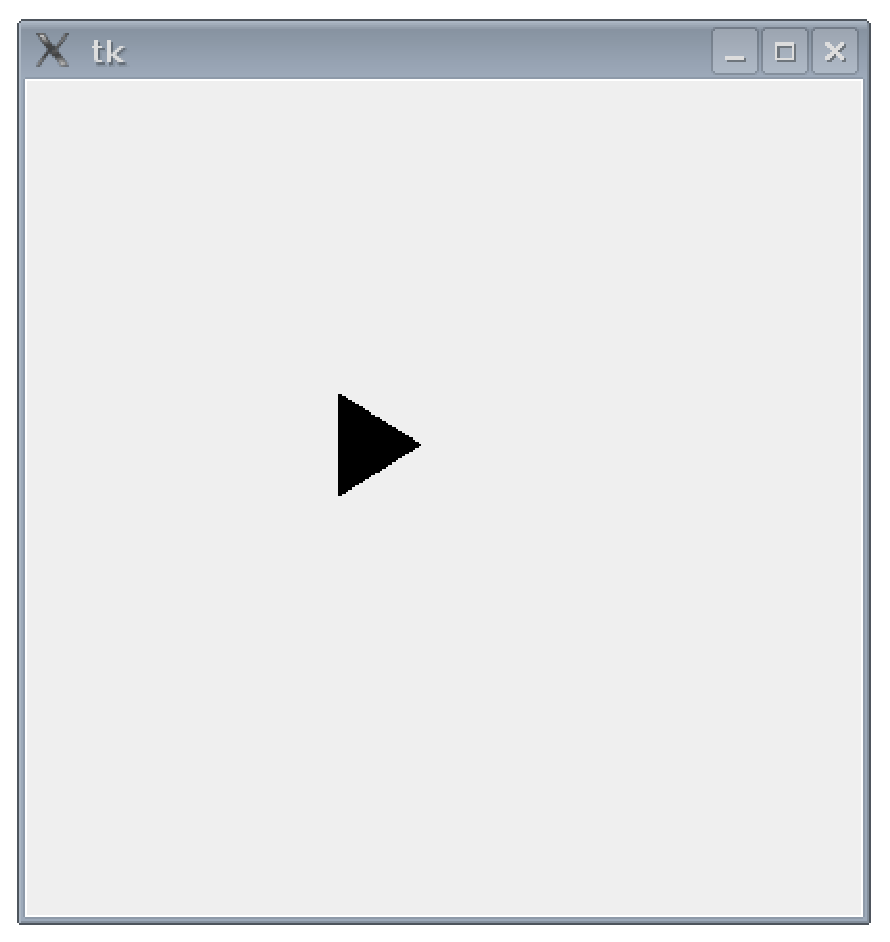
\includegraphics[width=80mm]{figure45.eps}
\end{center}
\caption{Triángulo moviéndose en diagonal hacia abajo de la pantalla.}\label{fig45}
\end{figure}

\section{Reaccionando a los eventos$\ldots$}\index{módulos!Tkinter!eventos}

Podemos hacer que el triángulo reaccione cuando se pulsa una tecla. Para ello es necesario utilizar una cosa que se llama \emph{enlace a eventos}\footnote{En inglés lo llaman `event bindings'}.  Los eventos son cosas que pueden pasar mientras el programa se está ejecutando, por ejemplo: mover el ratón, pulsar una tecla, o cerrar una ventana. Puedes hacer que el módulo \code{Tk} `vigile' estos eventos, y que haga algo como respuesta a ellos.  Para comenzar a `manejar' eventos necesitamos empezar creando una función.  Imagina que lo que queremos hacer es mover el triángulo cuando se pulse la tecla Intro. Podemos definir una función para mover el triángulo:

\begin{listing}
\begin{verbatim}
>>> def mover_triangulo(event):
...     lienzo.move(1, 5, 0)
\end{verbatim}
\end{listing}

Es obligatorio que si la función sirve para manejar eventos reciba un único parámetro (el evento), este parámetro le sirve al módulo Tk para enviar informacion a la función sobre lo que ha pasado.

Lo siguiente que hacemos es decirle a Tk que esta función es la que se debe utilizar para `manejar' un evento concreto. Para ello se utiliza la función del lienzo \code{bind\_all}\index{módulos!Tkinter!bind\_all}. El código completo es como sigue:

\begin{listing}
\begin{verbatim}
>>> from Tkinter import *
>>> ventana = Tk()
>>> lienzo = Canvas(ventana, width=400, height=400)
>>> lienzo.pack()
>>> lienzo.create_polygon(10, 10, 10, 60, 50, 35)
>>> def mover_triangulo(evento):
...     lienzo.move(1, 5, 0)
...
>>> lienzo.bind_all('<KeyPress-Return>', mover_triangulo)
\end{verbatim}
\end{listing}

El primer parámetro de la función \code{bind\_all} describe el evento que queremos que Tk atienda.  En este caso el evento es \code{$<$KeyPress$-$Return$>$} (que es la pulsación -KeyPress- de la tecla Intro -Return-).  Además, el segundo parámetro indica la función que queremos que se ejecute cada vez que suceda el evento indicado. En este caso decimos que se llame a la función \code{mover\_triangulo}.

Si ejecutas este código pulsa primero en el lienzo con el ratón para asegurarte de que está activada esa ventana, luego pulsa la tecla Intro (Return) en el teclado.

¿Qué te parecería cambiar la dirección del triángulo dependiendo de la tecla que se pulse, por ejemplo, las teclas de flecha?  Primero vamos a modificar la función \code{move} a lo siguiente:

\begin{listing}
\begin{verbatim}
>>> def mover_triangulo(evento):
...     if evento.keysym == 'Up':
...         lienzo.move(1, 0, -3)
...     elif evento.keysym == 'Down':
...         lienzo.move(1, 0, 3)
...     elif evento.keysym == 'Left':
...         lienzo.move(1, -3, 0)
...     elif evento.keysym == 'Right':
...         lienzo.move(1, 3, 0)
\end{verbatim}
\end{listing}

El objeto evento que se pasa como parámetro a la función contiene un conjunto de \emph{propiedades}\footnote{Las propiedades son valores con nombre que describen algo de un objeto---por ejemplo, una propiedad del cielo es que es azul (algunas veces), una propiedad de un coche es que tiene ruedas. En términos de programación, una propiedad tiene un nombre y un valor. Hasta cierto punto son como variables que pertenecen a un objeto.}. Una de estas propiedades es \code{keysym} que es una cadena con el nombre de la tecla que se ha pulsado.  Si la propiedad contiene la cadena `Up', ejecutamos la función move con -3 en el eje y, lo que hace que se mueva hacia arriba; si contiene el texto `Down' sumamos 3 al eje y, lo que hace que se mueva hacia abajo. Lo mismo se hace para la izquierda y para la derecha.  Recuerda que el primer parámetro es el número que identifica la la figura que se quiere mover en el lienzo, el segundo valor a sumar al eje x (coordenada horizontal), y el último parámetro es el valor a sumar al eje y (coordenada vertical).  Lo siguiente que hacemos es decirle a Tk que use la misma función mover\_triangulo para manejar los eventos de las cuatro teclas de flecha (Arriba, abajo, izquierda y derecha). El código ahora queda así:

\begin{listingignore}
\begin{verbatim}
>>> from Tkinter import *
>>> ventana = Tk()
>>> lienzo = Canvas(ventana, width=400, height=400)
>>> lienzo.pack()
>>> lienzo.create_polygon(10, 10, 10, 60, 50, 35)
1
>>> def mover_triangulo(evento):
...     if evento.keysym == 'Up':
...         lienzo.move(1, 0, -3)
...     elif evento.keysym == 'Down':
...         lienzo.move(1, 0, 3)
...     elif evento.keysym == 'Left':
...         lienzo.move(1, -3, 0)
...     elif evento.keysym == 'Right':
...         lienzo.move(1, 3, 0)
...
>>> lienzo.bind_all('<KeyPress-Up>', mover_triangulo)
>>> lienzo.bind_all('<KeyPress-Down>', mover_triangulo)
>>> lienzo.bind_all('<KeyPress-Left>', mover_triangulo)
>>> lienzo.bind_all('<KeyPress-Right>', mover_triangulo)
\end{verbatim}
\end{listingignore}

\noindent
Su pruebas este ejemplo, observarás que el triángulo se mueve ahora en la dirección de la tecla de flecha que pulses.

\newpage
